\lab{Differentiation}{Differentiation}
\label{lab:Derivatives}
\objective{Derivatives are central in many applications.
Depending on the application and on the available information, the derivative may be calculated symbolically, numerically, or with differentiation software.
In this lab we explore these three ways to take a derivative, discuss what settings they are each appropriate for, and demonstrate their strengths and weaknesses.
% This lab should be done after completing the Python Essentials lab on SymPy.
}

\section*{Symbolic Differentiation} % =========================================

The derivative of a known mathematical function can be calculated symbolically with SymPy.
This method is the most precise way to take a derivative, but it is computationally expensive and requires knowing the closed form formula of the function.
Use \li{sy.diff()} to take a symbolic derivative.

\begin{lstlisting}
>>> import sympy as sy

>>> x = sy.symbols('x')
>>> sy.diff(x**3 + x, x)     # Differentiate x^3 + x with respect to x.
<<3*x**2 + 1>>
\end{lstlisting}

\begin{problem}
Write a function that defines $f(x) = (\sin(x) + 1)^{\sin(\cos(x))}$ and takes its symbolic derivative with respect to $x$ using SymPy.
Lambdify the resulting function so that it can accept NumPy arrays and return the resulting function handle.
% returns the derivative of $e^{\sin\left(\cos\left(x\right)\right)}$ at $x=1$ as a float using SymPy.

To check your function, plot $f$ and its derivative $f'$ over the domain $[-\pi, \pi]$.
It may be helpful to move the bottom spine to $0$ so you can see where the derivative crosses the $x$-axis.
\begin{lstlisting}
>>> from matplotlib import pyplot as plt

>>> ax = plt.gca()
>>> ax.spines["bottom"].set_position("zero")
\end{lstlisting}
% >>> for label in ["right", "top"]:      # Turn other spines off.
% ...     ax.spines[label].set_visible(False)
% ...
% \end{lstlisting}
\label{prob:sympy-symbolic-diff}
\end{problem}

\section*{Numerical Differentiation} % ========================================

% Derivatives can be approximated numerically by formulas called \emph{finite difference quotients}.
% Although these formulas do not return exact answers like SymPy, they are computationally inexpensive.
% They are especially advantageous in situations where the original function may not be known or when the using derivative is very complex.

One definition for the derivative of a function $f:\mathbb{R}\rightarrow\mathbb{R}$ at a point $x_0$ is
\[
f'(x_0) = \lim_{h\rightarrow 0} \frac{f(x_0 + h)-f(x_0)}{h}.
\]
Since this definition relies on $h$ approaching $0$, choosing a small, fixed value for $h$ approximates $f'(x_0)$:
\begin{equation}
f'(x_0) \approx \frac{f(x_0+h) - f(x_0)}{h}.
\label{eq:first-order-forward-difference}
\end{equation}
This approximation is called the \emph{first order forward difference quotient}.
Using the points $x_0$ and $x_0-h$ in place of $x_0+h$ and $x_0$, respectively, results in the \emph{first order backward difference quotient},
\begin{equation}
f'(x_0) \approx \frac{f(x_0) - f(x_0-h)}{h}.
\label{eq:first-order-backward-difference}
\end{equation}

Forward difference quotients use values of $f$ at $x_0$ and points greater than $x_0$, while backward difference quotients use the values of $f$ at $x_0$ and points less than $x_0$.
A \emph{centered difference quotient} uses points on either side of $x_0$, and typically results in a better approximation than the one-sided quotients.
Combining (\ref{eq:first-order-forward-difference}) and (\ref{eq:first-order-backward-difference}) yields the \emph{second order centered difference quotient},
\[
f'(x_0) = \frac{1}{2}f'(x_0) + \frac{1}{2}f'(x_0) \approx
\frac{f(x_0+h) - f(x_0)}{2h} + \frac{f(x_0) - f(x_0-h)}{2h}
= \frac{f(x_0+h) - f(x_0-h)}{2h}.
\]

\begin{figure}[H] % Show which points each quotient uses.
\centering
    \begin{tikzpicture}
    % Define colors
    % Create asterisks and name each point
    \foreach \p/\x in {a/-5,b/-4,c/-3,d/-2,e/-1,f/0,g/1,h/2,i/3,j/4,k/5}{\node[text depth=.25ex,text height=3ex] (\p) at (\x,0) {\textbf{*}};}
    % Circles
    \draw[thick,blue!30!black,opacity=0.5] (a) circle (7pt);
    \draw[thick,blue!30!black,opacity=0.5] (f) circle (7pt);
    \draw[thick,blue!30!black,opacity=0.5] (k) circle (7pt);
    % Arrows and labels below
    \draw[->,>=stealth',thick,blue,shorten >=-.1cm,text=black] (-5,-1) node[text=black,below,font=\normalsize,opacity=1,align=center] {$f'(\bar{x})$\\Forward Difference} -- (a);
    \draw[->,>=stealth',thick,green,shorten >=-.1cm] (0,-1) node[text=black,below,font=\normalsize,opacity=1,align=center] {$f'(\hat{x})$\\Centered Difference} -- (f);
    \draw[->,>=stealth',thick,red,shorten >=-.1cm] (5,-1) node[text=black,below,font=\normalsize,opacity=1,align=center] {$f'(\tilde{x})$\\Backward Difference} -- (k);
    % Labels above
    \foreach \s/\t in {a/\bar{x},b/\bar{x}+h,e/\hat{x}-h,f/\hat{x},g/\hat{x}+h,j/\tilde{x}-h,k/\tilde{x}}{\node[anchor=south,yshift=.5cm,text depth=.25ex,text height=1.5ex] at (\s) {$\t$};}
    % Background rectangles
    \begin{pgfonlayer}{background}
    \draw[ultra thick,draw=blue,fill=blue,opacity=0.2] (-5.5,.5) rectangle +(2,-1);
    \draw[ultra thick,draw=green,fill=green,opacity=0.2] (-1.5,.5) rectangle +(3,-1);
    \draw[ultra thick,draw=red,fill=red,opacity=0.2] (5.5,.5) rectangle +(-2,-1);
    \end{pgfonlayer}
    \end{tikzpicture}
\caption{} % The different types of difference quotients require evaluating the function at different points near the point of interest.}
\label{fig:difference-quotient-grid}
\end{figure}

\begin{info}
The finite difference quotients in this section all approximate the first derivative of a function.
The terms \emph{first order} and \emph{second order} refers to how quickly the approximation converges on the actual value of $f'(x_0)$ as $h$ approaches $0$, not to how many derivatives are being taken.

There are finite difference quotients for approximating higher order derivatives, such as $f''$ or $f'''$.
For example, the centered difference quotient
\[
f''(x_0) \approx \frac{f(x_0-h) - 2f(x_0) + f(x_0+h)}{h^2}
\]
approximates the second derivative.
This particular quotient is important for finite difference methods that approximate numerical solutions to some partial differential equations.
\end{info}


While we do not derive them here, there are other finite difference quotients that use more points to approximate the derivative, some of which are listed below.
Using more points generally results in better convergence properties.

\begin{table}[H]
\centering
\begin{tabular}{|c|c|c|}
\hline
Type & Order & Formula \\
\hline \multirow{6}{*}{Forward} & & \\
    & 1 & \Large{$\frac{f(x_0+h) - f(x_0)}{h}$} \\
    & & \\
    \cline{2-3} & & \\
    & 2 & \Large{$\frac{-3f(x_0) + 4f(x_0+h) - f(x_0+2h)}{2h}$} \\
    & & \\
\hline \multirow{6}{*}{Backward} & & \\
    & 1 & \Large{$\frac{f(x_0) - f(x_0-h)}{h}$} \\
    & & \\
    \cline{2-3} & & \\
    & 2 & \Large{$\frac{3f(x_0) - 4f(x_0-h) + f(x_0-2h)}{2h}$} \\
    & & \\
\hline \multirow{6}{*}{Centered} & & \\
    & 2 & \Large{$\frac{f(x_0+h) - f(x_0-h)}{2h}$} \\
    & & \\
    \cline{2-3} & & \\
    & 4 & \Large{$\frac{f(x_0-2h) - 8f(x_0-h) + 8f(x_0+h) -f(x_0+2h)}{12h}$} \\
    & & \\
\hline
\end{tabular}
\caption{Common finite difference quotients for approximating $f'(x_0)$.}
\label{table:finite-difference-quotients}
\end{table}

\begin{problem} % Implement finite difference quotients.
Write a function for each of the finite difference quotients listed in Table \ref{table:finite-difference-quotients}.
Each function should accept a function handle $f$, an array of points \li{x}, and a float $h$; each should return an array of the difference quotients evaluated at each point in \li{x}.

To test your functions, approximate the derivative of $f(x) = (\sin(x) + 1)^{\sin(\cos(x))}$ at each point of a domain over $[-\pi,\pi]$.
Plot the results and compare them to the results of Problem \ref{prob:sympy-symbolic-diff}.
\label{prob:implement-finite-difference-quotients}
\end{problem}

\subsection*{Convergence of Finite Difference Quotients} % --------------------

Finite difference quotients are typically derived using Taylor's formula.
This method also shows how the accuracy of the approximation increases as $h\rightarrow 0$:
\begin{equation}
f(x_0+h) = f(x_0) + f'(x_0)h + R_2(h)
\quad\Longrightarrow\quad
\frac{f(x_0+h) - f(x_0)}{h} - f'(x_0) = \frac{R_2(h)}{h},
\label{eq:taylor-formula-forward-diff}
\end{equation}
where $R_2(h) = h^2 \int_0^1 (1-t) f''(x_0+th)\:dt$.
Thus the absolute error of the first order forward difference quotient is
\[
\left| \frac{R_2(h)}{h} \right|
= |h| \left|\int_0^1 (1 - t)f''(x_0+th)\:dt\right|
\leq |h| \int_0^1 |1 - t||f''(x_0+th)|\:dt.
\]
If $f''$ is continuous, then for any $\delta > 0$, setting $M = \sup_{x \in (x_0-\delta, x_0+\delta)} f''(x)$ guarantees that
\[
\left | \frac{R_2(h)}{h} \right | \leq |h|\int_0^1 M dt = M|h|\hspace{0.03in}{\in}\hspace{0.03in}O(h).
\]
whenever $|h| < \delta$.
That is, the error decreases at the same rate as $h$.
If $h$ gets twice as small, the error does as well.
This is what is meant by a \emph{first order} approximation.
In a \emph{second order} approximation, the absolute error is $O(h^2)$, meaning that if $h$ gets twice as small, the error gets four times smaller.

\begin{info} % O(h^2) notation
The notation $O(f(n))$ is commonly used to describe the temporal or spatial complexity of an algorithm.
In that context, a $O(n^2)$ algorithm is much worse than a $O(n)$ algorithm.
However, when referring to error, a $O(h^2)$ algorithm is \textbf{better} than a $O(h)$ algorithm because it means that the accuracy improves faster as $h$ decreases.
\end{info}

\begin{problem} % Convergence of difference quotients.
Write a function that accepts a point $x_0$ at which to compute the derivative of $f(x) = (\sin(x)+1)^{\sin(\cos(x))}$.
Use your function from Problem \ref{prob:sympy-symbolic-diff} to compute the exact value of $f'(x_0)$.
Then use each your functions from Problem \ref{prob:implement-finite-difference-quotients} to get an approximate derivative $\tilde{f}'(x_0)$ for $h=10^{-8},10^{-7},\ldots,10^{-1},1$.
Track the absolute error $|f'(x_0) - \tilde{f}'(x_0)|$ for each trial, then plot the absolute error against $h$ on a log-log scale (use \li{plt.loglog()}).

Instead of using \li{np.linspace()} to create an array of $h$ values, use \li{np.logspace()}.
This function generates logarithmically spaced values between two powers of $10$.
\begin{lstlisting}
>>> import numpy as np
>>> np.logspace(-3, 0, 4)           # Get 4 values from 1e-3 to 1e0.
array([ 0.001,  0.01 ,  0.1  ,  1.   ])
\end{lstlisting}

For $x_0 = 1$, your plot should resemble the following figure.
\begin{figure}[H]
    \centering
    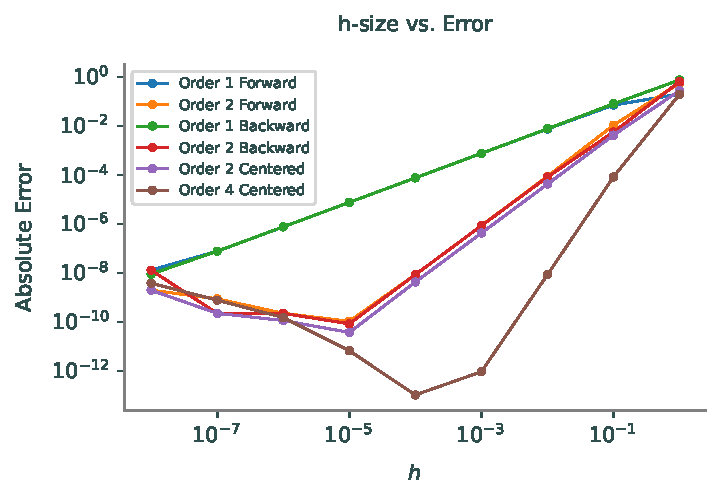
\includegraphics[width=.7\textwidth]{figures/error_plot.pdf}
\end{figure}
\label{prob:difference-quotient-convergence}
\end{problem}

\begin{warn}
Mathematically, choosing smaller $h$ values results in tighter approximations of $f'(x_0)$.
However, Problem \ref{prob:difference-quotient-convergence} shows that when $h$ gets too small, the error stops decreasing.
This numerical error is due to the denominator in each finite difference quotient becoming very small.
The optimal value of $h$ is usually one that is small, but not too small.
\end{warn}

\begin{problem}
The radar stations $A$ and $B$, separated by the distance $a = 500$ m, track a plane $C$ by recording the angles $\alpha$ and $\beta$ at one-second intervals.
Your goal, back at air traffic control, is to determine the speed of the plane.%
\footnote{This problem is adapted from an exercise in \cite{kiusalaas2013numerical}.}
%
\begin{figure}[H]
    \includegraphics[width=.5\textwidth]{figures/plane_diagram.png}
\end{figure}
%
Let the position of the plane at time $t$ be given by $(x(t),y(t))$.
The speed at time $t$ is the magnitude of the velocity vector, $\|\frac{d}{dt}(x(t),y(t))\| = \sqrt{x'(t)^2 + y'(t)^2}$.
The closed forms of the functions $x(t)$ and $y(t)$ are unknown (and may not exist at all), but we can still use numerical methods to estimate $x'(t)$ and $y'(t)$.
For example, at $t=3$, the second order centered difference quotient for $x'(t)$ is
\[
x'(3) \approx \frac{x(3+h) - x(3-h)}{2h} = \frac{1}{2}(x(4) - x(2)).
\]
In this case $h=1$ since data comes in from the radar stations at $1$ second intervals.

Successive readings for $\alpha$ and $\beta$ at integer times $t=7,8,\ldots,14$ are stored in the file \texttt{plane.npy}.
Each row in the array represents a different reading; the columns are the observation time $t$, the angle $\alpha$ (in degrees), and the angle $\beta$ (also in degrees), in that order.
The Cartesian coordinates of the plane can be calculated from the angles $\alpha$ and $\beta$ as follows.
\begin{equation}
\label{eq:differentiation-plane-conversion}
x(\alpha, \beta) = a \frac{\tan(\beta)}{\tan(\beta)-\tan(\alpha)}
\qquad
y(\alpha, \beta) = a \frac{\tan(\beta)\tan(\alpha)}{\tan(\beta)-\tan(\alpha)}
\end{equation}
Load the data, convert $\alpha$ and $\beta$ to radians, then compute the coordinates $x(t)$ and $y(t)$ at each given $t$ using \ref{eq:differentiation-plane-conversion}.
Approximate $x'(t)$ and $y'(t)$ using a first order forward difference quotient for $t=7$, a first order backward difference quotient for $t=14$, and a second order centered difference quotient for $t=8,9,\ldots,13$ (see Figure \ref{fig:difference-quotient-grid}).
Return the values of the speed $\sqrt{x'(t)^2+y'(t)^2}$ at each $t$.
\\(Hint: \li{np.deg2rad()} will be helpful.)
\end{problem}

\subsection*{Numerical Differentiation in Higher Dimensions} % ================

Finite difference quotients can also be used to approximate derivatives in higher dimensions.
The \emph{Jacobian matrix} of a function $f:\mathbb{R}^n \rightarrow \mathbb{R}^m$ at a point $\x_0 \in \mathbb{R}^n$ is the $m \times n$ matrix $J$ whose entries are given by
\begin{equation*}
J_{ij} = \frac{\partial f_i}{\partial x_j}(\x_0).
\end{equation*}
For example, the Jacobian for a function $f:\mathbb{R}^3 \rightarrow \mathbb{R}^2$ is defined by
\[
J = \left[\begin{array}{c|c|c}
\arrayrulecolor{gray}
\frac{\partial f}{\partial x_1}&\frac{\partial f}{\partial x_2}&\frac{\partial f}{\partial x_3}
\end{array}\right]
=
\left[\begin{array}{ccc}
\frac{\partial f_1}{\partial x_1}&\frac{\partial f_1}{\partial x_2}&\frac{\partial f_1}{\partial x_3}
\\ \\
\frac{\partial f_2}{\partial x_1}&\frac{\partial f_2}{\partial x_2}&\frac{\partial f_2}{\partial x_3}
\end{array}\right],
\qquad
\text{where}
\qquad
f(\x) =
\left[\begin{array}{c}
f_1(\x) \\ f_2(\x)
\end{array}\right],
\quad
\x = \left[\begin{array}{c}
x_1 \\ x_2 \\ x_3
\end{array}\right].
\]

The difference quotients in this case resemble directional derivatives.
The first order forward difference quotient for approximating a partial derivative is
\[
\frac{\partial f}{\partial x_j}(\x_0) \approx \frac{f(\x_0 + h\e_j) - f(\x_0)}{h},
\]
where $\e_j$ is the $j$th standard basis vector.
The second order centered difference approximation is
\begin{equation}
\frac{\partial f}{\partial x_j}(\x_0) \approx \frac{f(\x_0 + h\e_j) - f(\x_0 - h\e_j)}{2h}.
\label{eq:centered-quotient-high-dimension}
\end{equation}

\begin{problem}
Write a function that accepts a function $f:\mathbb{R}^n\rightarrow\mathbb{R}^m$, a point $\x_0 \in \mathbb{R}^n$, and a float $h$.
Approximate the Jacobian matrix of $f$ at $\x$ using the second order centered difference quotient in (\ref{eq:centered-quotient-high-dimension}).
\\(Hint: the standard basis vector $\e_j$ is the $j$th column of the $n\times n$ identity matrix $I$.)

To test your function, define a simple function like $f(x,y) = [x^2, x^3 - y]\trp$ where the Jacobian is easy to find analytically, then check the results of your function against SymPy or your own scratch work.
\label{prob:jac_center}
\end{problem}

\begin{comment} % Not enough room. Needs updating if added back in.
\begin{problem}
Find the error between your Jacobian function and the analytically computed derivative on the square $[-1,1] \times [-1,1]$ using ten thousand grid points (100 per side).
You may apply your Jacobian function to the points one at a time using a double \li{for} loop.  Once you get the error matrix for a given point, calculate the Frobenius norm of this matrix (\li{la.norm()} defaults to the Frobenius norm).  This norm will be your total error for that point.
Return the maximum error of your Jacobian function over all points in the square.

Hint: The following code defines the function
$f(x,y) = \left[\begin{array}{c} x^2 \\ x+y \end{array}\right]$.

\begin{lstlisting}
# f accepts a length-2 NumPy array
>>> f = lambda x: np.array([x[0]**2, x[0]+x[1]])
\end{lstlisting}
\end{problem}
\end{comment}

% TODO: Introduce Google tangent as well as HIPS Autograd. Be brief.

\section*{Differentiation Software} % =========================================

Many machine learning algorithms and structures, especially neural networks, rely on the gradient of a cost or objective function.
To facilitate their research, several organizations have recently developed Python packages for numerical differentiation.
For example, the Harvard Intelligent Probabilistic Systems Group (HIPS) started developing \li{autograd} in 2014 (\url{https://github.com/HIPS/autograd}) and Google 
created JAX (\url{https://github.com/google/jax}) as a successor to \li{autograd}.
Popular deep learning libraries also contain automatic differentiation libraries.
These tools use an algorithm known as \emph{automatic differentiation} that is incredibly robust: they can differentiate functions with NumPy routines, \li{if} statements, \li{while} loops, and even recursion.
% They are therefore beneficial for calculating derivatives of unconventional or very complex functions.

We conclude with a brief introduction to JAX.
JAX is not included in Anaconda.
It can be installed as follows on Mac and Linux:
\begin{lstlisting}
pip install "jax[cpu]"
\end{lstlisting}
Installation directly via \li{pip} is not currently supported on Windows, however.
Some unofficial builds for Windows are available at \url{https://github.com/cloudhan/jax-windows-builder}.
JAX also has additional installation options that allow it to do computations on a GPU using the CUDA library.
See \url{https://github.com/google/jax#installation} for additional options for these cases.


JAX's \li{grad()} accepts a scalar-valued function and returns its gradient as a function that accepts the same parameters as the original.
To support most of the NumPy features, JAX comes with its own thinly-wrapped version of Numpy, \li{jax.numpy}.
Import this version of NumPy as \li{jnp} to avoid confusion.

\begin{lstlisting}
>>> from jax import numpy as jnp            # Use JAX's version of NumPy.
>>> from jax import grad

>>> g = lambda x: jnp.exp(jnp.sin(jnp.cos(x)))
>>> dg = grad(g)                            # dg() is a callable function.
>>> dg(1.)                                  # Use floats as input, not ints.
DeviceArray(-1.2069776, dtype=float32, weak_type=True)
\end{lstlisting}

\begin{comment} % Not enough room, and not useful later.
JAX can differentiate a function as many times as desired.

\begin{lstlisting}
>>> f = lambda x: jnp.sin(x) + 3**jnp.cos(x)

# Calculate the first derivative.
>>> df = grad(f)

# Calculate the second derivative and so forth.
>>> ddf = grad(df)
>>> dddf = grad(ddf)
>>> dddf(1.)
2.683445898750351
\end{lstlisting}
\end{comment}

Functions that \li{grad()} produces do not support array broadcasting, meaning they do not accept arrays as input.
The easiest way to create a function is to use \li{jnp.vectorize()} on the derivative.
%Autograd's \li{elementwise_grad()} returns functions that can accept arrays, like using \li{"numpy"} as an argument in SymPy's \li{sy.lambdify()}.

\begin{lstlisting}
>>> pts = jnp.array([1, 2, 3], dtype=<<float>>)
>>> dg = jnp.vectorize(grad(g))        # Calculate g'(x) with array support.
>>> dg(pts)                            # Evaluate g'(x) at each of the points.
DeviceArray([-1.2069776 , -0.5551414 , -0.03356146], dtype=float32)
\end{lstlisting}

% >>> g = lambda x: anp.exp(anp.sin(anp.cos(x)))
% >>> g(pts)                          # Evaluate g(x) at an array of points.
% array([ 1.67262669,  0.66748447,  0.43343135])


SymPy would have no trouble differentiating $g(x)$ in these examples.
However, JAX can also differentiate Python functions that look nothing like traditional mathematical functions.
For example, the following code computes the Taylor series of $e^{x}$ with a loop.

\begin{lstlisting}
>>> from sympy import factorial

>>> def taylor_exp(x, tol=.0001):
...     """Compute the Taylor series of e^x with terms greater than tol."""
...     result, i, term = 0, 0, 1
...     while jnp.abs(term) > tol:
...         term = x**i / int(factorial(i))
...         result, i = result + term, i + 1
...     return result
...
>>> d_exp = grad(taylor_exp)
>>> d_exp(2., .1), d_exp(2., .0001)
(DeviceArray(7.266667, dtype=float32, weak_type=True),
 DeviceArray(7.3889947, dtype=float32, weak_type=True))
\end{lstlisting}

\begin{problem} % Take the derivative of a recursive function.
The \emph{Chebyshev Polynomials} satisfy the recursive relation
\[
T_0(x) = 1,\qquad T_1(x) = x,\qquad T_n(x) = 2xT_{n-1}(x) - T_{n-2}(x).
\]
Write a function that accepts an array $x$ and an integer $n$ and recursively computes $T_n(x)$.
Use JAX and your first function to create a function for $T_n'(x)$.
Use this last function to plot each $T_n'(x)$ over the domain $[-1, 1]$ for $n=0,1,2,3,4$.
\\(Hint: Use \li{jnp.ones_like(x)} to handle the case when $n = 0$.)
\end{problem}

\begin{problem} % Compare differentiation methods.
Let $f(x) = (\sin(x) + 1)^{\sin(\cos(x))}$ as in Problems \ref{prob:sympy-symbolic-diff} and \ref{prob:difference-quotient-convergence}.
Write a function that accepts an integer $N$ and performs the following experiment $N$ times.
\begin{enumerate}
\item Choose a random value $x_0$.
\item Use your function from Problem \ref{prob:sympy-symbolic-diff} to calculate the ``exact'' value of $f'(x_0)$.
Time how long the entire process takes, including calling your function (each iteration).
\item Time how long it takes to get an approximation $\tilde{f}'(x_0)$ of $f'(x_0)$ using the fourth-order centered difference quotient from Problem \ref{prob:difference-quotient-convergence}.
Record the absolute error $|f'(x_0) - \tilde{f}'(x_0)|$ of the approximation.
\item Time how long it takes to get an approximation $\bar{f}'(x_0)$ of $f'(x_0)$ using JAX (calling \li{grad()} every time).
Record the absolute error $|f'(x_0) - \bar{f}'(x_0)|$ of the approximation.
\end{enumerate}

Plot the computation times versus the absolute errors on a log-log plot with different colors for SymPy, the difference quotient, and JAX.
For SymPy, assume an absolute error of \li{1e-18} (since only positive values can be shown on a log plot).

For $N=200$, your plot should resemble the following figure.
Note that SymPy has the least error but longer computation time, and that the difference quotient takes the least amount of time but has the most error.
%JAX might be considered a ``happy medium,'' a least for this problem.
JAX, on the other hand, does not appear to be as well-suited to this particular problem.
However, for more complicated functions and functions of multiple variables, it tends to be a ``happy medium'' between the two, with faster runtime than SymPy.

\begin{figure}[H]
    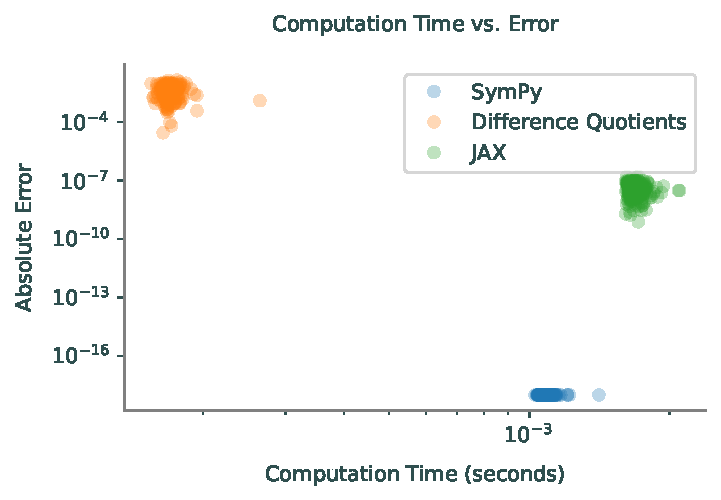
\includegraphics[width=.7\textwidth]{figures/efficiency.pdf}
    \caption{Solution with $N = 200$.}
\end{figure}
\end{problem}

\newpage

\section*{Additional Material} % ==============================================

\subsection*{More JAX} % -------------------------------------------------

For scalar-valued functions with multiple inputs, the parameter \li{argnums} specifies the variable that the derivative is computed with respect to.
Providing a list for \li{argnums} gives several outputs.

\begin{lstlisting}
>>> f = lambda x,y: 3*x*y + 2*y - x

# Take the derivative of f with respect to the first variable, x.
>>> dfdx = grad(f, argnums=0)            # Should be dfdx(x,y) = 3y - 1,
>>> dfdx(5., 1.)                        # so dfdx(5,1) = 3 - 1 = 2.
DeviceArray(2., dtype=float32, weak_type=True)

# Take the gradient with respect to the second variable, y.
>>> dfdy = grad(f, argnums=1)            # Should be dfdy(x,y) = 3x + 2,
>>> dfdy(5., 1.)                        # so dfdy(5,1) = 15 + 2 = 17.
DeviceArray(17., dtype=float32, weak_type=True)

# Get the full gradient.
>>> grad_f = grad(f, argnums=[0,1])
>>> jnp.array(grad_f(5., 1.))
DeviceArray([ 2., 17.], dtype=float32)
\end{lstlisting}

Finally, JAX's \li{jacobian()} can differentiate vector-valued functions.
% The following example shows how to find the Jacobian of $f(x,y) = \left[\begin{array}{c} x^2 \\ x+y \end{array}\right]$.

\begin{lstlisting}
>>> from jax import jacobian

>>> f = lambda x: jnp.array([x[0]**2, x[0]+x[1]])
>>> f_jac = jacobian(f)
>>> f_jac(jnp.array([1., 1.]))
DeviceArray([[2., 0.],
             [1., 1.]], dtype=float32)
\end{lstlisting}

% There used to be a section on Tangent, but it's now deprecated.

\begin{comment} % NOT FINISHED! ...and not really necessary.
\subsection*{Convergence of the Centered Difference Quotient} % ---------------

Recall from the proof of Taylor's theorem that $R_k = \frac{f^{(k)}(x_0)}{k!}h^k + R_{k+1}$.
Therefore,
\begin{align*}
\frac{R_2(-h) - R_2(h)}{2h} &= \frac{1}{2h}\left(\frac{f''(x_0)}{2!}h^2 + R_{3}(-h) - \frac{f''(x_0)}{2!}h^2 - R_{3}(h) \right)\\
&= \frac{1}{2h} ( R_3(-h)-R_3(h))\\
&= \frac{1}{2h}\left(  \left( \int_0^1 \frac{(1-t)^2}{2} f'''(x_0+th) dt \right) h^3  -  \left(\int_0^1 \frac{(1-t)^2}{2} f'''(x_0-th) dt \right) h^3  \right)\\
&= \left(  \int_0^1 \frac{(1-t)^2}{4}( f'''(x_0+th)-f'''(x_0-th)) \right)h^2\\
&{\in}\hspace{0.3in}O(h^2)
\end{align*}
once $h$ is restricted to some $\delta$-neighborhood of 0.
So this centered difference quotient is of the second order and its error is smaller than using the first order forward and backward difference quotients when $|h|<1$.
\end{comment}

% =============================================================================
% OLD IMAGE FILTER MATERIAL (might work well in Fourier 2 lab?) ===============
% =============================================================================

\begin{comment}
\section*{Image Filters} % ====================================================

Recall that a computer stores an image as a 2-D array of pixel values (i.e., a matrix of intensities).
An image filter is a function that transforms an image by operating on it locally.
That is, to compute the $ij$th pixel value in the new image, an image filter uses only the pixels in a small neighborhood around the $ij$th pixel in the original image.

In this lab, we will use a filter derived from the gradient of an image to find edges in an image.

\subsection*{Convolutions} % --------------------------------------------------

One example of an image filter is to \emph{convolve} an image with a filter matrix.
A filter matrix is a matrix whose height and width are relatively small odd numbers.
If the filter matrix is
\[
F = \begin{array}
f_{-1,-1}&f_{-1,0}&f_{-1,1}\\
f_{0,-1}&f_{0,0}&f_{0,1}\\
f_{1,-1}&f_{1,0}&f_{1,1}
\end{array},
\]
then the convolution of an image $A$ with $F$ is $A \ast F = (C_{ij})$ where
\begin{equation}\label{equ:convolve}
C_{ij} = \sum_{k=-1}^1 \sum_{\ell=-1}^1 f_{k\ell}A_{i+k,j+\ell}.
\end{equation}
Say $A$ is an $m \times n$ matrix. Here, we take $A_{ij}=0$ when $i \not \in \{1, \ldots m\}$ or $j \not \in \{1, \ldots, n\}$.
The value of $C_{ij}$ is a linear combination of the nearby pixel values, with coefficients given by $F$ (see Figure \ref{fig:convolution}).
In fact, $C_{ij}$ equals the Frobenius inner product of $F$ with the $3 \times 3$ submatrix of $A$ centered at $ij$.

\begin{figure}
\centering
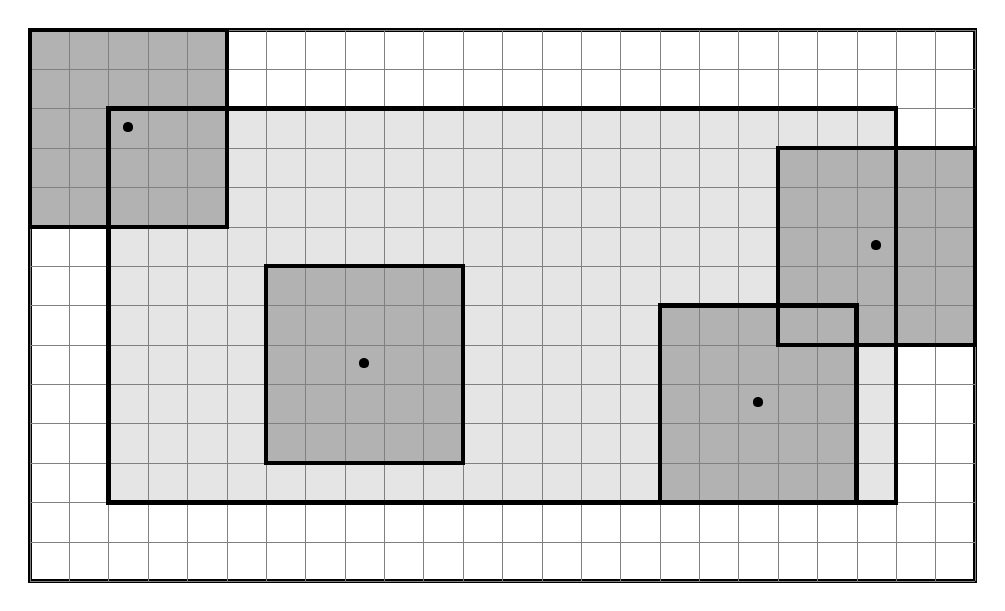
\begin{tikzpicture}
\node[draw, minimum width=12cm, minimum height=
    7cm, ultra thick](outer_rec)[]{};
\node[draw, minimum width=10cm, minimum height=
    5cm, ultra thick, fill=black!10!](inner_rec)[]{};
\node[draw, minimum width=2.5cm, minimum height=2.5cm,
    ultra thick, fill=black!30!](square1)at(-4.75,2.25){\textbullet};
\node[draw, minimum width=2.5cm, minimum height=2.5cm,
    ultra thick,fill=black!30!](square2)at(-1.75,-.75){\textbullet};
\node[draw, minimum width=2.5cm, minimum height=2.5cm,
    ultra thick, fill=black!30!](square3)at(4.75,.75){\textbullet};
\node[draw, minimum width=2.5cm, minimum height=2.5cm,
    ultra thick, fill=black!30!](square4)at(3.25,-1.25){\textbullet};
\draw[step=.5, ultra thin, color=black!50!](-6,-3.5)grid(6,3.5);

\node[draw, minimum width=10cm, minimum height=
    5cm, ultra thick, ][]{};
\node[draw, minimum width=2.5cm, minimum height=2.5cm,
    ultra thick]at(-4.75,2.25){};
\node[draw, minimum width=2.5cm, minimum height=2.5cm,
    ultra thick]at(-1.75,-.75){};
\node[draw, minimum width=2.5cm, minimum height=2.5cm,
    ultra thick]at(4.75,.75){};
\node[draw, minimum width=2.5cm, minimum height=2.5cm,
    ultra thick]at(3.25,-1.25){};
\end{tikzpicture}
\caption{This diagram illustrates how to convolve an image with a filter.
The light grey rectangle represents the original image $A$, and the dark grey squares are the filter $F$.
The larger rectangle is the image padded with zeros; i.e., all pixel values in the outer white band are 0.
To compute the entry of the convolution matrix $C$ located at a black dot, take the inner product of $F$ with the submatrix of the padded image centered at the dot.}
\label{fig:convolution}
\end{figure}

\subsubsection*{Implementation in NumPy} % - - - - - - - - - - - - - - - - - -

Let us write a function that convolves an image with a filter.
You can test this function on the image \li{cameraman.jpg}, which appears in Figure \ref{fig:cameraman}.
The following code loads this image and plots it with matplotlib.

\begin{lstlisting}
>>> image = plt.imread('cameraman.jpg')
>>> plt.imshow(image, cmap = 'gray')
>>> plt.show()
\end{lstlisting}

Here is the function definition and some setup.

\begin{lstlisting}
1. def Filter(image, F):
2.     m, n = image.shape
3.     h, k = F.shape
\end{lstlisting}

To convolve \li{image} with the filter \li{F}, we must first \emph{pad} the array \li{image} with zeros around the edges.
This is because in \eqref{equ:convolve}, entries $A_{ij}$ are set to zero when $i$ or $j$ is out of bounds.
We do this by creating a larger array of zeros, and then making the interior part of the array equal to the original image (see Figure \ref{fig:convolution}).

For example, if the filter is a $3 \times 3$ matrix, then the following code will pad the matrix with the appropriate number of zeros.

\begin{lstlisting}
 # Create a larger matrix of zeros
image_pad = np.zeros((m+2, n+2))
# Make the interior of image_pad equal to the original image
image_pad[1:1+m, 1:1+n] = image
\end{lstlisting}

We want to do this in general in our function.  Note that the number of zeros we need to pad our array depends on the size of the filter \li{F}.

\begin{lstlisting}
5.    image_pad = # Create an array of zeros of the appropriate size
6.   # Make the interior of image_pad equal to image
\end{lstlisting}

Finally, we iterate through the image to compute each entry of the convolution matrix.

\begin{lstlisting}
7.    C = np.zeros(image.shape)
8.    for i in range(m):
9.        for j in range(n):
10.            C[i,j] = # Compute C[i, j]
\end{lstlisting}

\subsubsection*{Gaussian Blur} % - - - - - - - - - - - - - - - - - - - - - - -

A \emph{Gaussian blur} is an image filter that operates on an image by convolving with the matrix
\[
G = \frac{1}{159}\begin{array}
2&4&5&4&2\\
4&9&12&9&4\\
5&12&15&12&5\\
4&9&12&9&4\\
2&4&5&4&2
\end{array}.
\]

Blurring an image can remove ``noise'', or random variation that is the visual analog of static in a radio signal (and equally undesirable).

\begin{problem}\label{prob:filter}
\leavevmode
Finish writing the function \li{Filter} by filling in lines 5, 6, and 10.  Hint: Note in \ref{equ:convolve}, $C_{ij}$ was calculated by summing from -1 to 1.  This is only the case if the filter \li{F} is $3 \times 3$. A slight modification is needed in the general case.  Test your function on the image \li{cameraman.jpg} using the Gaussian Blur. The result is in Figure \ref{fig:cameraman_blur}.
\end{problem}

\begin{figure}
\centering
\begin{subfigure}[b]{.49\textwidth}
\centering
\includegraphics[width=\textwidth]{figures/cameraman.jpg}
\caption{Unfiltered image.}
\label{fig:cameraman}
\end{subfigure}
\begin{subfigure}[b]{.49\textwidth}
\centering
\includegraphics[width=\textwidth]{figures/cameramanBlur.pdf}
\caption{Image after Gaussian blur is applied.}
\label{fig:cameraman_blur}
\end{subfigure}
\begin{subfigure}[b]{.49\textwidth}
\centering
\includegraphics[width=\textwidth]{figures/edges.pdf}
\caption{Image after the Sobel filter is applied.}
\label{fig:cameraman_edges}
\end{subfigure}
\caption{Here is an example of a Gaussian blur and the Sobel filter applied to an image.
This photo, known as ``cameraman,'' is a standard test image in image processing.
A database of such images can be downloaded from \url{http://www.imageprocessingplace.com/root_files_V3/image_databases.htm}.}
\label{fig:cameraman1}
\end{figure}

\subsection*{Edge Detection} % ------------------------------------------------

Automatic detection of edges in an image can be used to segment or sharpen the image.
We will find edges with the Sobel filter, which computes the gradient of the image at each pixel.
The magnitude of the gradient tells us the rate of change of the pixel values, and so large magnitudes should
correspond to edges within the image.
The Sobel filter is not a convolution, although it does use convolutions.

We can think of an image as a function from a $2 \times 2$ grid of points to $\mathbb{R}$.
The image maps a pixel location to an intensity.
It does not make sense to define the derivative of this function as a limit because the domain is discrete---a step size $h$ cannot take on arbitrarily small values.
Instead, we \emph{define} the derivative to be the centered difference quotient of the previous section.
That is, we define the derivative in the $x$-direction at the $ij$th pixel to be
\[
\frac{1}{2}A_{i+1, j} - \frac{1}{2}A_{i-1, j}.
\]

We can use a convolution to create a matrix $A_x$ whose $ij$th entry is the derivative of $A$ at the $ij$th entry, in the $x$-direction.
In fact, $A_x = A \ast S$, where
\[
S = \frac{1}{8}
\left[\begin{array}{ccc}
-1 & 0 & 1\\
-2 & 0 & 2\\
-1 & 0 & 1
\end{array}\right].
\]

Note that this convolution takes a weighted average of the $x$-derivatives at $(i, j)$, $(i, j+1)$, and $(i, j-1)$.
The derivative at $(i, j)$ is weighted by 2.
Using a weighted average instead of just the derivative at $(i, j)$ makes the derivative less affected by noise.

Now we can define the Sobel filter.
A Sobel filter applied to an image $A$ results in an array $B = (B_{ij})$ of 0's and 1's, where the 1's trace out the edges in the image.
By definition,
\[
B_{ij} = \left\{
     \begin{array}{ll}
       1 & \text{if}\; \;\|\nabla A(ij)\|_2 > M \\
       0 & \text{otherwise}.
     \end{array}
   \right.
\]
Here, $\nabla A(ij) = ((A \ast S)_{ij}, (A\ast S^T)_{ij})$ is the gradient of $A$ at the $ij$th pixel.
The constant $M$ should be ``sufficiently large'' enough to pick out those pixels with the largest gradient (i.e., those pixels that are part of an edge).
A good choice for $M$ is 4 times the average value of $\|\nabla A(ij)\|_2$ over the whole image $A$.

When the Sobel filter is applied to \li{cameraman.jpg}, we get the image in Figure \ref{fig:cameraman_edges}.
Here, the 1's in $B$ were mapped to ``white'' and the 0's were mapped to ``black.''

\begin{problem}
Write a function that accepts an image as input and applies the Sobel filter to the image.  Test your function on \li{cameraman.jpg}.  Hint: If you want to find the average of a matrix \li{A}, use the function \li{A.mean()}.
\end{problem}
\end{comment}
